\section*{Process Management}
\begin{description}
  \item[Process] Program loaded into mem, in execution
  \item[Program] Passive entity stored on disk
  \item[Process states] new, ready, running, waiting, terminated
  \item[Process Control Block] Information about each P: P state, P number, PID, program counter, CPU registers, Mem.-management information (allocated mem for process), I/O status, CPU scheduling info (e.g. priority), Accounting info (e.g. CPU used)
  \item[Context Switch] When CPU switches to another P, save PCB of prev. P, load PCB of new P.
\end{description}
% 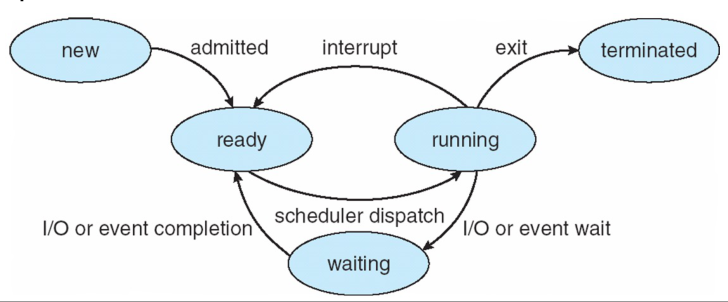
\includegraphics[width=0.5\linewidth]{process_state.png}
\subsection*{Processes Layout}
\begin{description}
  \item[Stack] temporary data: function parameters, return addresses, local variables
  \item[Heap] dynamically mem allocated during execution
  \item[data] Global variables
  \item[text] executable code
\end{description}
\subsection*{Operations on processes}
\begin{description}
  \item[Process creation]Parent P creates child (fork()) which can create own children → tree structure, every proc. has a unique P identifier (pid). Either parent and child share all, a part or no resources.
  \item[Process termination] P's delete themselves w/ exit(). Parent deletes child w/ abort(). Parent waits for child to end w/ wait(). child → \textbf{zombie} if child terminates w/o or before parent wait(), child → \textbf{orphan} if parent terminates.
\end{description}
\subsection*{Interprocess communication}
\begin{description}
  \item[Shared Memory]Communication is under control of user P (not OS), P's share mem. space. Issue: Producer-Consumer problem.
    % NOTE:producer-consumer problem defined in synchronization?
  \item[Message passing] Communication controlled by OS, Messaging b/w P's without shared variables.
  \item[Direct Message passing] A link is established b/w P's. They must name each other explicitly (send(P,message), receive(Q,message)). Only one communication link.
  \item[Indirect message passing] Messages are sent and received from mailboxes (i.e. ports). May share several communication links
  \item[Ordinary Pipe] Communication b/w parent and child, cannot be accessed from outside the proc. that created it. Have a read end (fd[1]) and write end (fd[0]). Exists until proc. completion.
  \item[Named Pipe, FIFO] Several P's can use pipe for communication. Exist until deleted. Appears as a file.
  \item[Socket] Endpoint of communication between different machines, concatination of IP and port. Data is sent via packets.
\end{description}
